\newpage
\section{Aufbau des neuronalen Netzes}

In diesem Abschnitt wird erklärt, wie unser neuronales Netz aufgebaut ist. Vor allem die Abbildung \ref{AnordungMerkuPix} ist für das bessere Verständnis der Matlab-Skripte wichtig. In den Matlab-Skripten muss immer die Pixelanzahl und die Merkmalanzahl angegeben werden. Dabei handelt es sich immer um einen symmetrischen Aufbau. Ist die Merkmalanzahl gleich 5, dann gibt es 25 Merkmale (5 in x-Richtung und 5 in y-Richtung). Das gleiche gilt für die Pixelanzahl. Bei einer Pixelanzahl von 8 werden für jedes Merkmale 8 mal 8 Pixel angenommen. Bei einer Merkmalanzahl von 5 und einer Pixelanzahl von 8 wird also eine Pixelmatrix von 40 mal 40 Pixel erzeugt.

\begin{figure}[hbt]
	\centering
	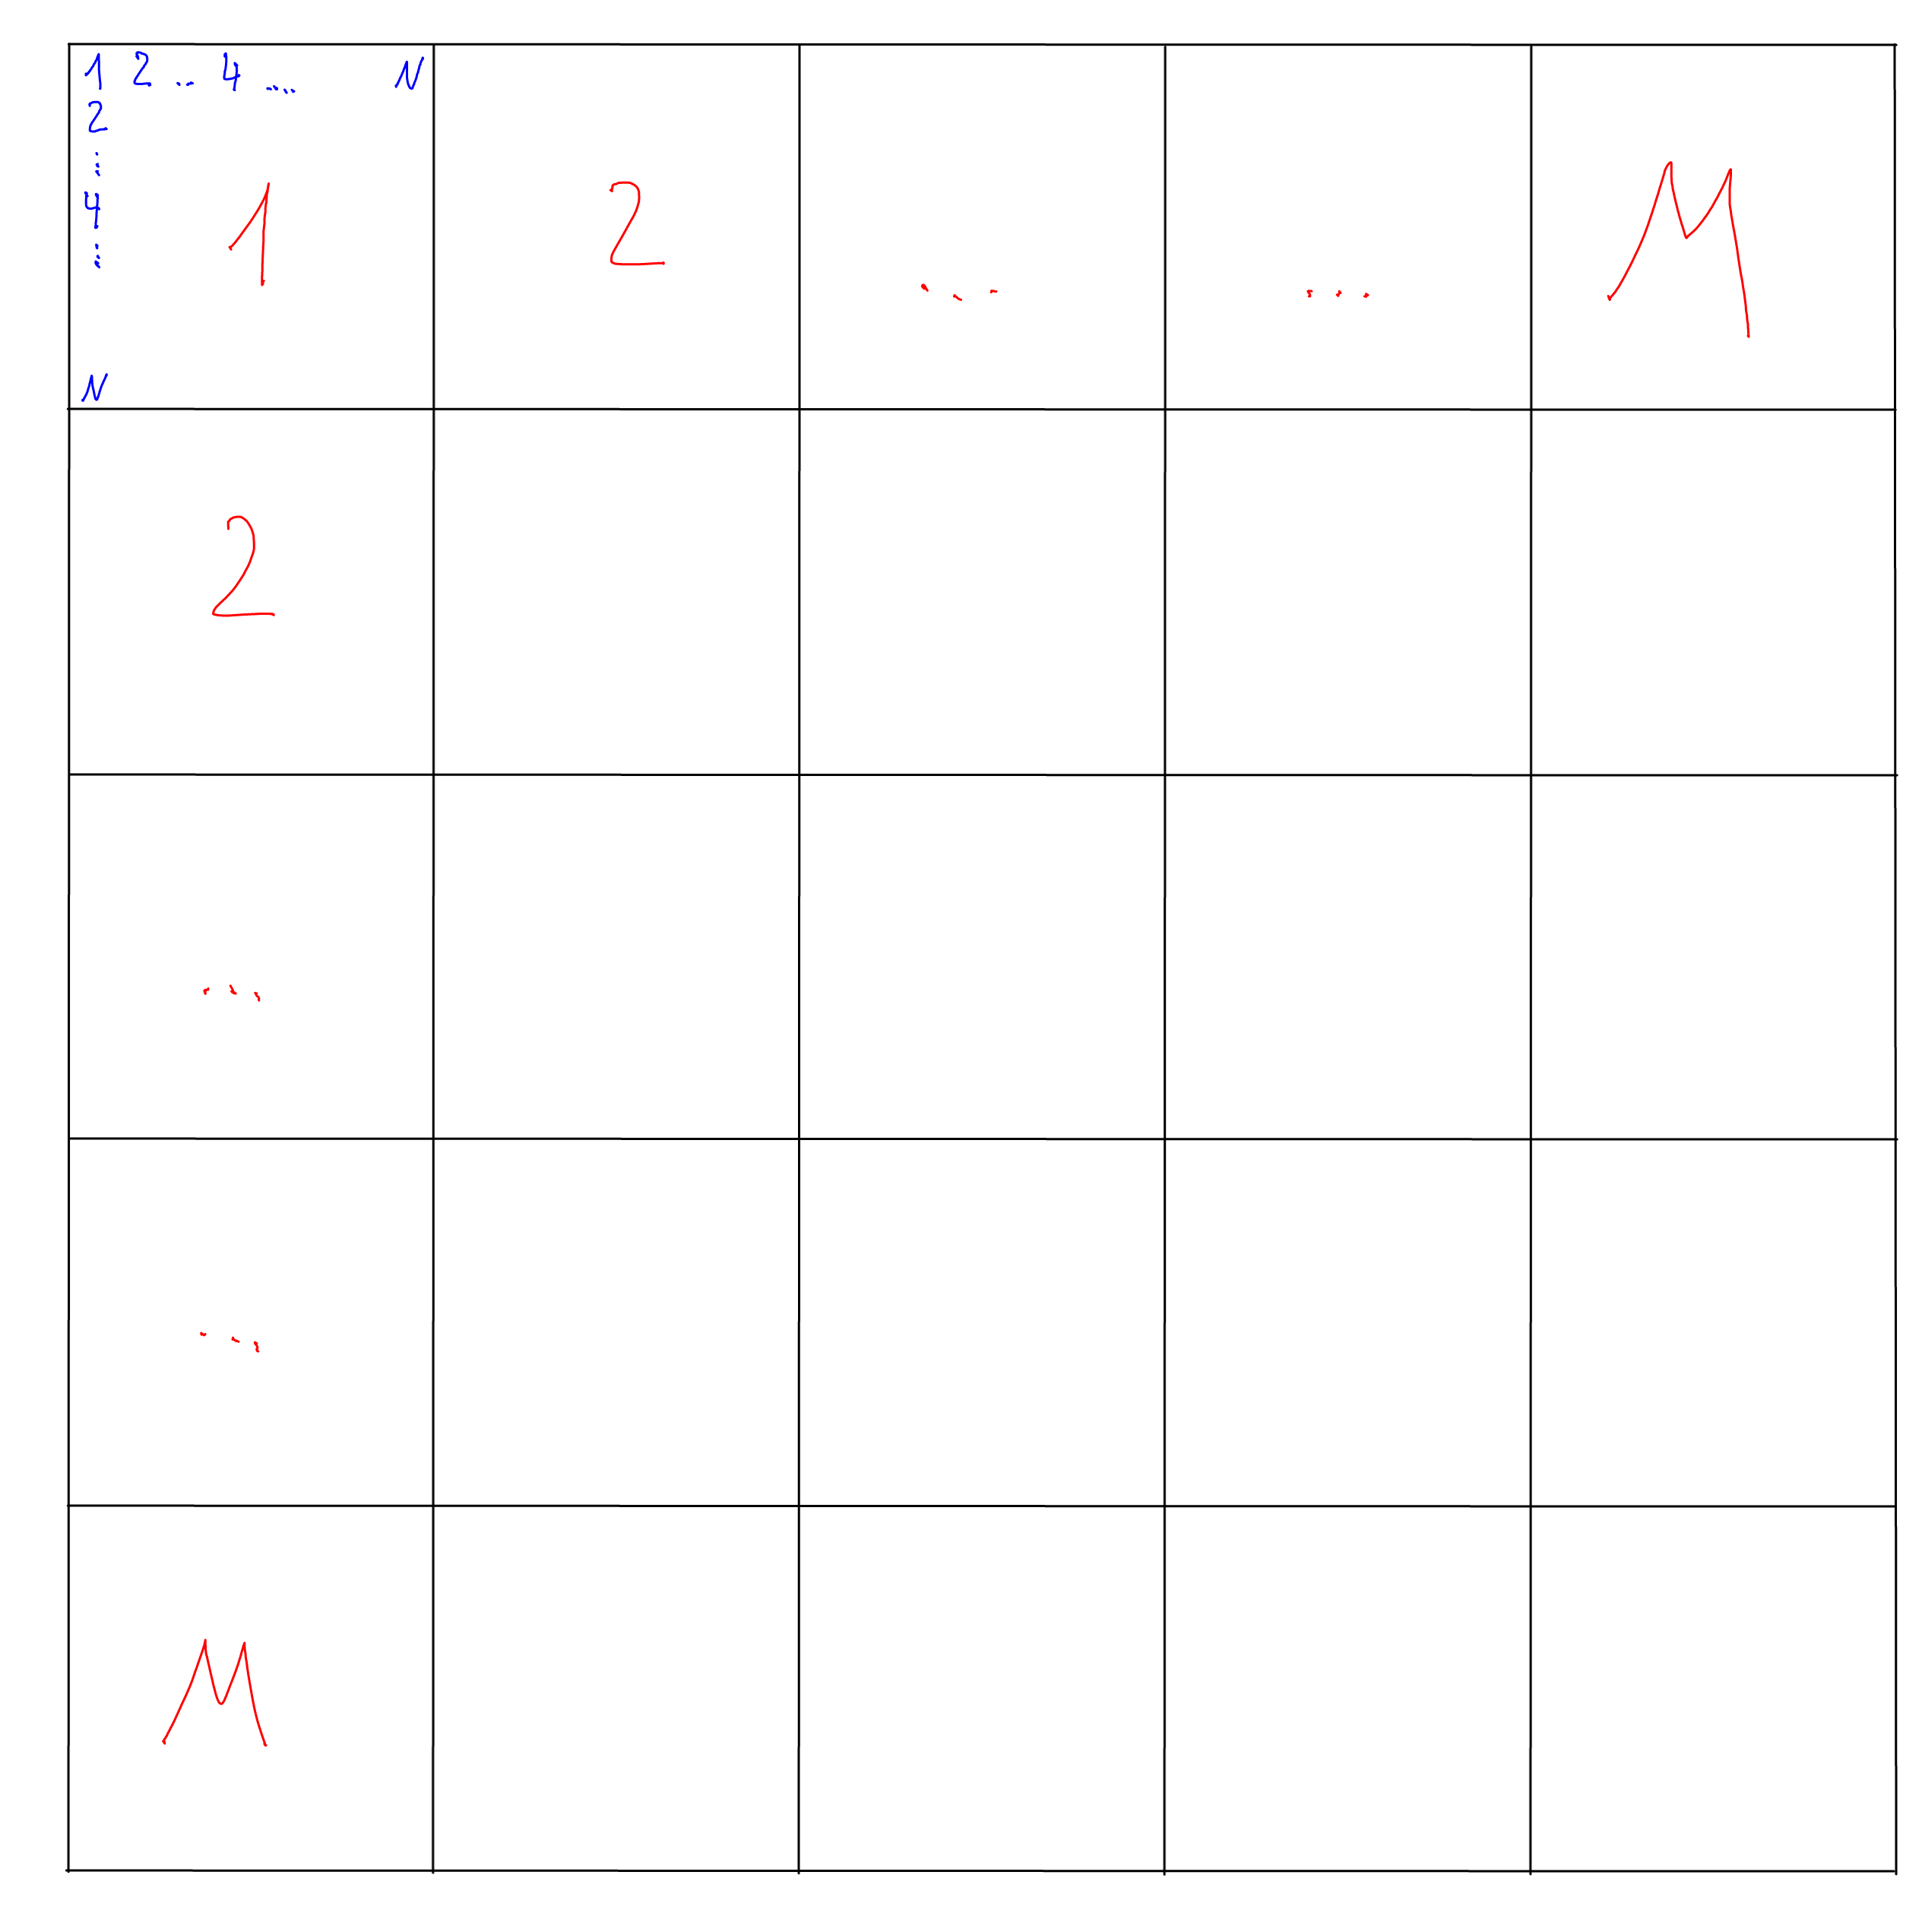
\includegraphics[width=0.5\linewidth]{./Bilder/Auswertung/Aufbau/page4}
	\caption{Anordnung der Merkmale und Pixel}
	\label{AnordungMerkuPix}
\end{figure}

In Abbildung \ref{Neuron1Ebene} ist ein Neuronenbeispiel abgebildet. Dieses Neuron der 1. Ebene fasst ein komplettes Merkmal mit all seinen Pixel zusammen. Dieses Neuron hat also in unserem Beispiel 64 Eingänge und es gibt 25 solcher Neuronen.

\begin{figure}[hbt]
	\centering
	
\includegraphics[width=0.6\linewidth]{./Bilder/Auswertung/Aufbau/page5}
	\caption{Neuron der 1. Ebene}
	\label{Neuron1Ebene}
\end{figure}

Mit einer einzigen Ebene von Neuronen kann sehr viel erreicht werden. Allerdings ist für die Gesamtauswertung eine zweite von Vorteil, um zum Beispiel besser Fehler zu detektieren bei sehr viel Rauschen. Bevor wir uns die zweite Ebene der Neuronen angucken, werfen wir einen Blick auf die Abbildung \ref{Erl2Ebene}. Hier sind drei Arten von Merkmalen zu erkennen. Die fünf schwarzen Merkmale detektieren einen horizontalen Balken, die blauen Merkmale einen vertikalen Balken und die roten Merkmale können hohes Rauschen detektieren. Die roten Merkmale erlauben es, eine bessere Konfiguration des neuronalen Netzes zu finden.

\begin{figure}[hbt]
	\centering
	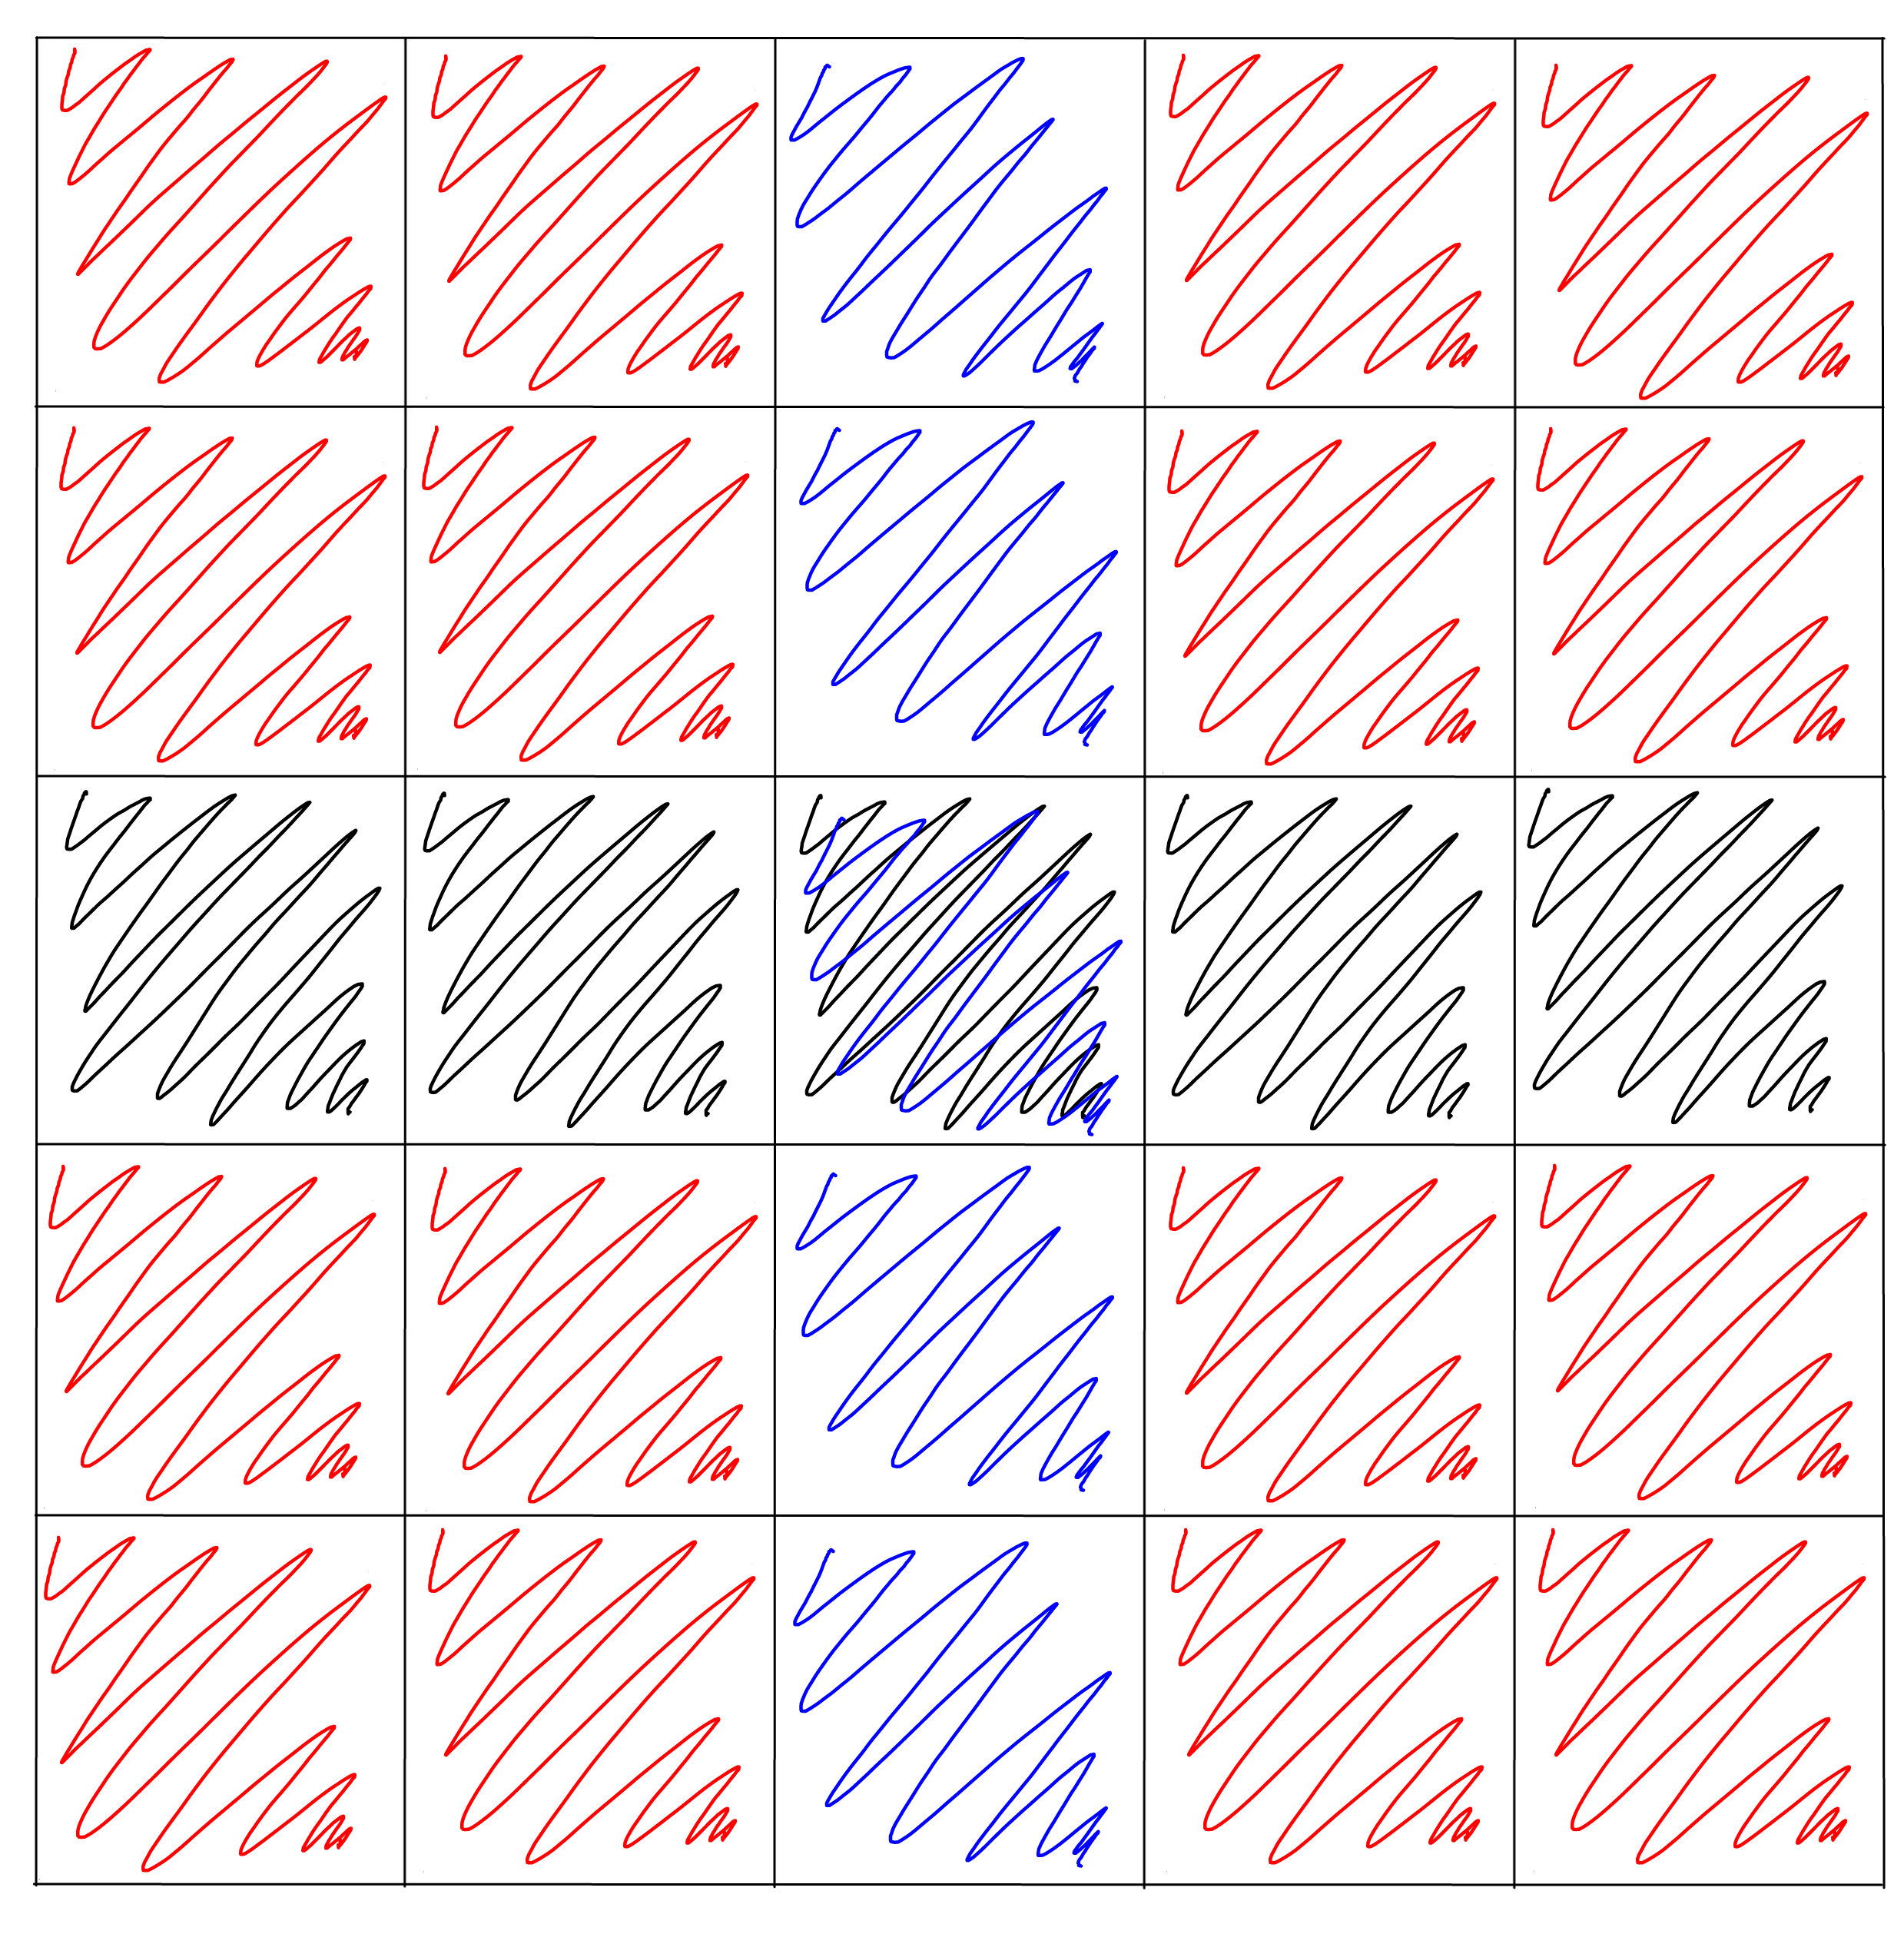
\includegraphics[width=0.6\linewidth]{./Bilder/Auswertung/Aufbau/page6}
	\caption{Erläuterung der Anordnung für die 2. Ebene}
	\label{Erl2Ebene}
\end{figure}

In Abbildung \ref{Neurin2Ebene} ist die komplette zweite Ebene des Neuronalen Netzes dargestellt. Alle drei Merkmale-Typen werden jeweils auf ein Neuron gegeben. In diesem Fall sind alle Gewichte auf eins gesetzt. Es muss nur der Bias eingestellt und eine Schwelle zur Detektion festgelegt werden. 

\begin{figure}[hbt]
	\centering
	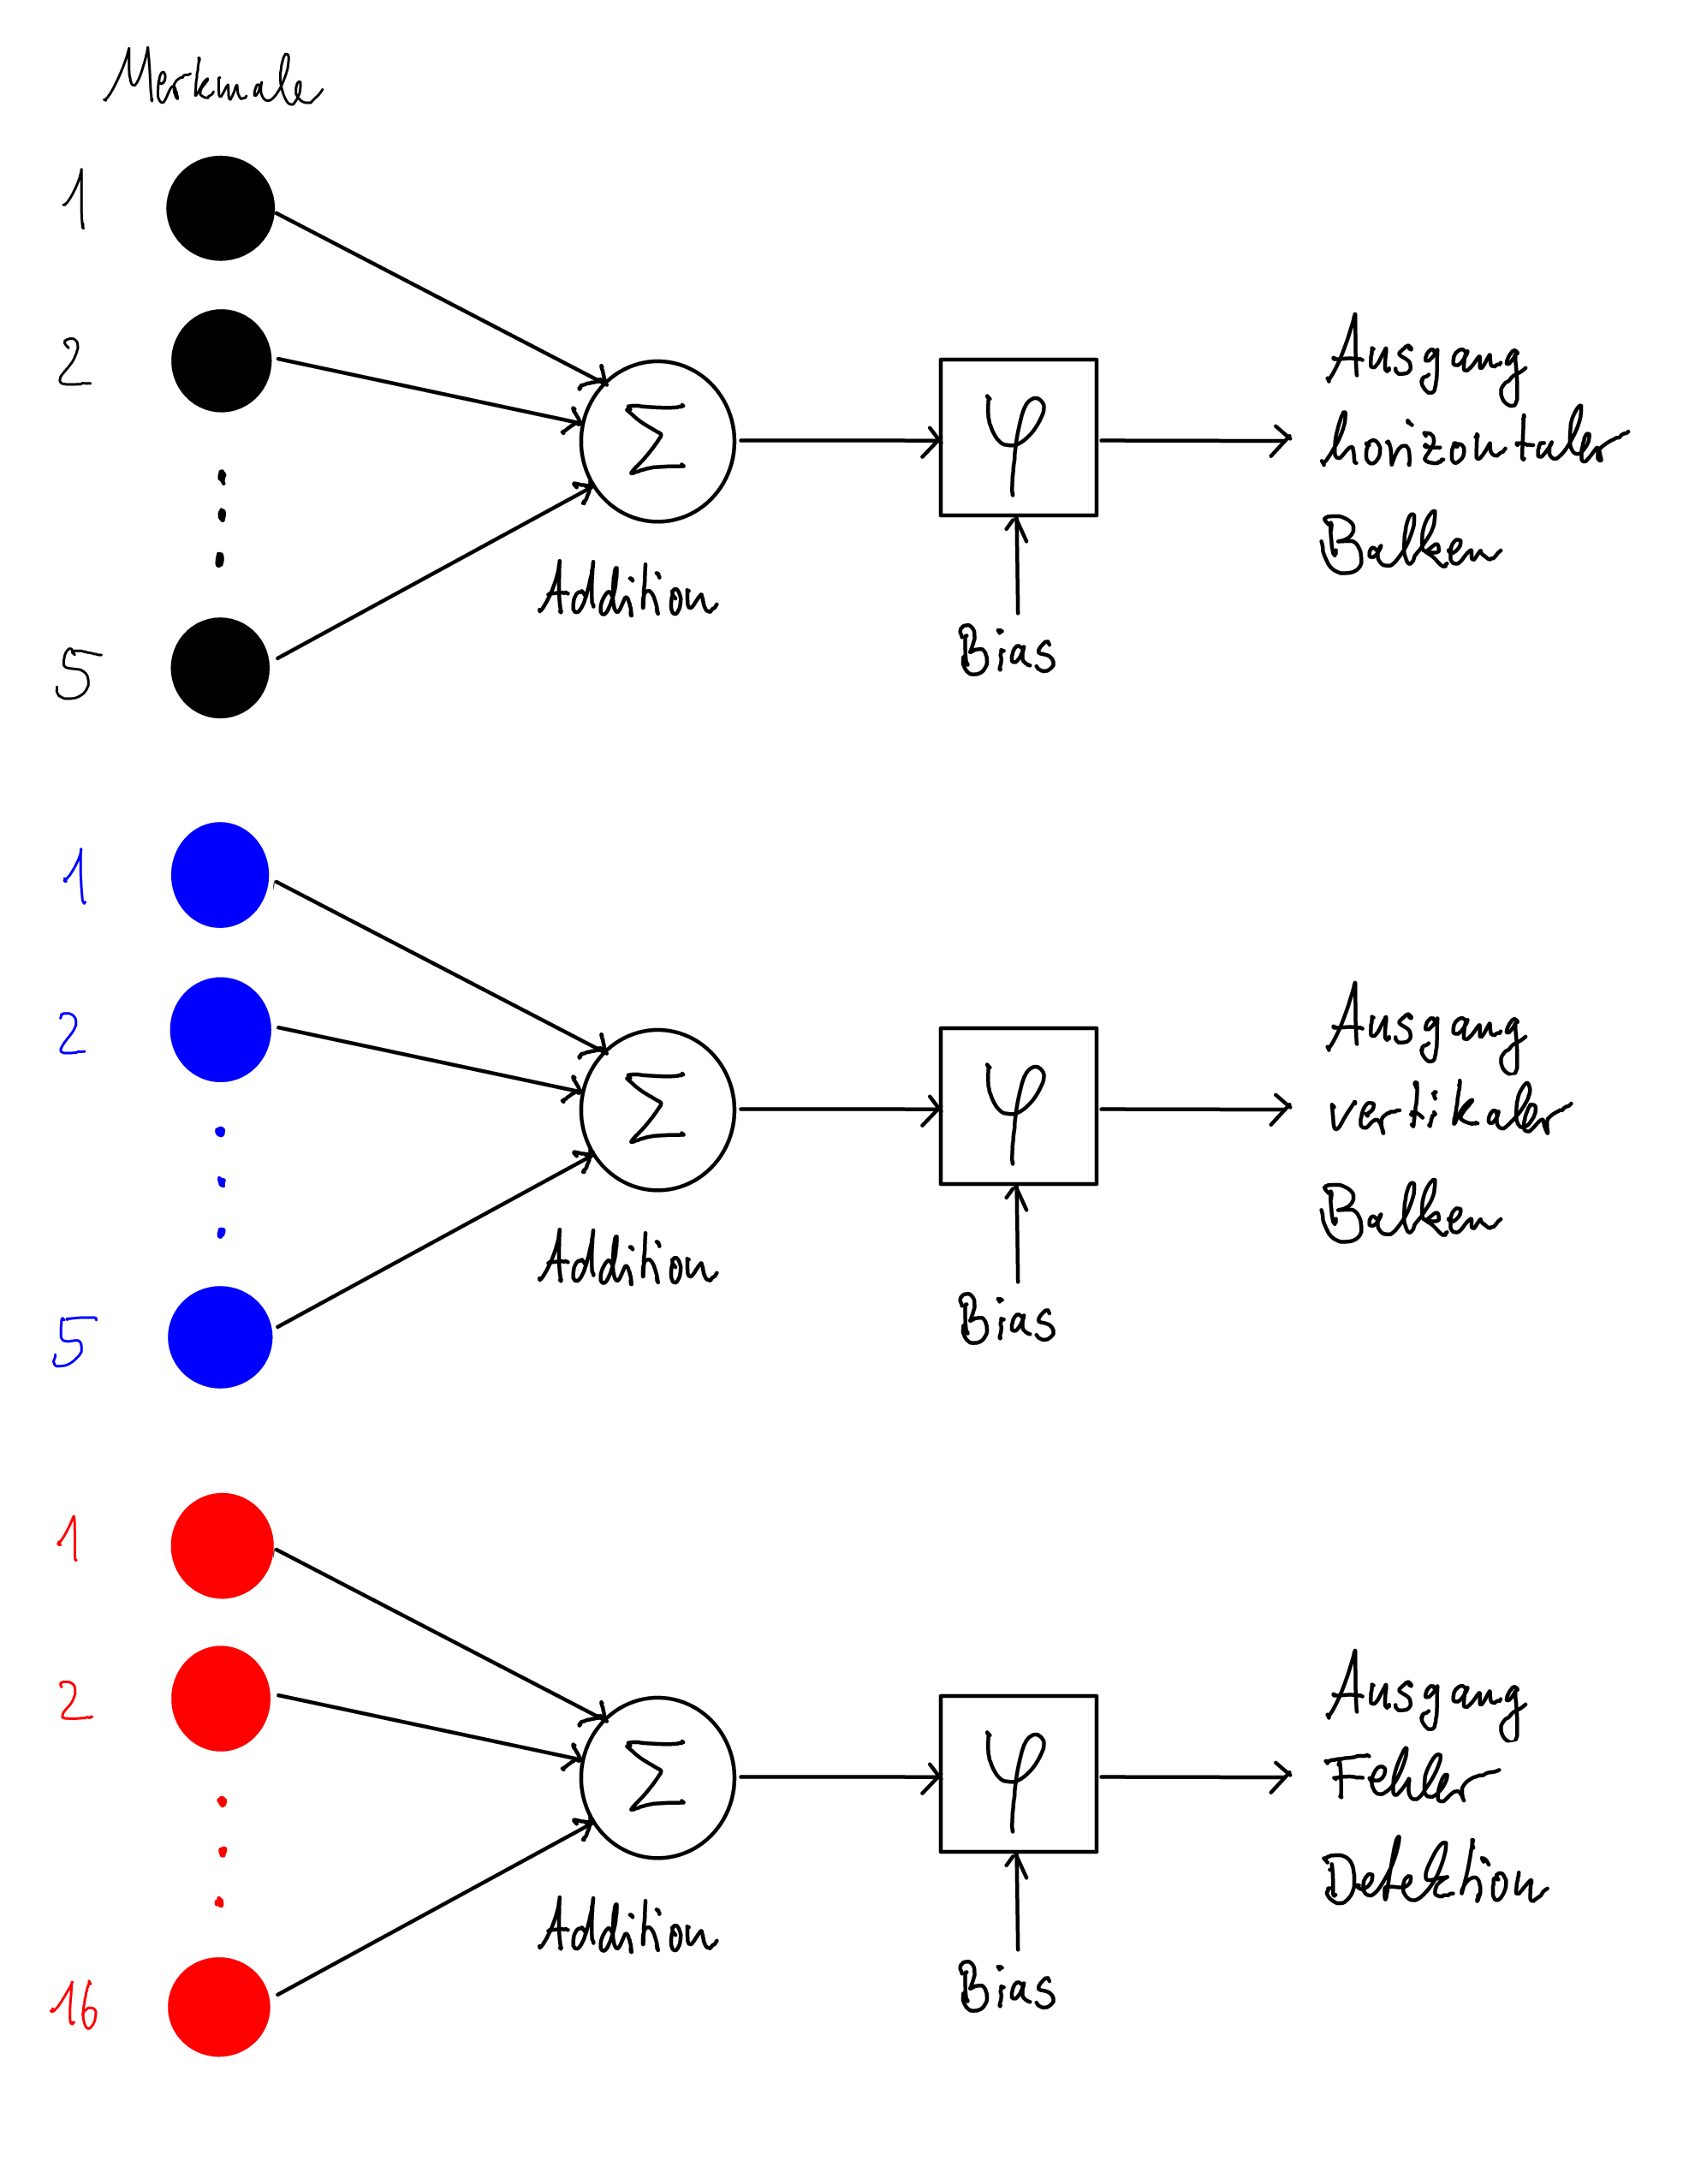
\includegraphics[width=0.8\linewidth]{./Bilder/Auswertung/Aufbau/page7}
	\caption{Neuronen der 2. Ebene}
	\label{Neurin2Ebene}
\end{figure}

Für die Auswertung der Neuronen der erste Ebene nutzen wir eine Sigmoid-Funktion. Für die zweite Ebene werden allerdings nicht die Ergebnisse der Sigmoid-Funktion weitergegeben, sondern die addierten Werte werden ohne eine weiteren Verarbeitung an die zweite Ebene weiter gegeben. Das entspricht einer linearen Aktivierungsfunktion mit dem Anstieg eins.

